\begin{figure}[H]
  \centering
  \hspace*{-1.5cm}
  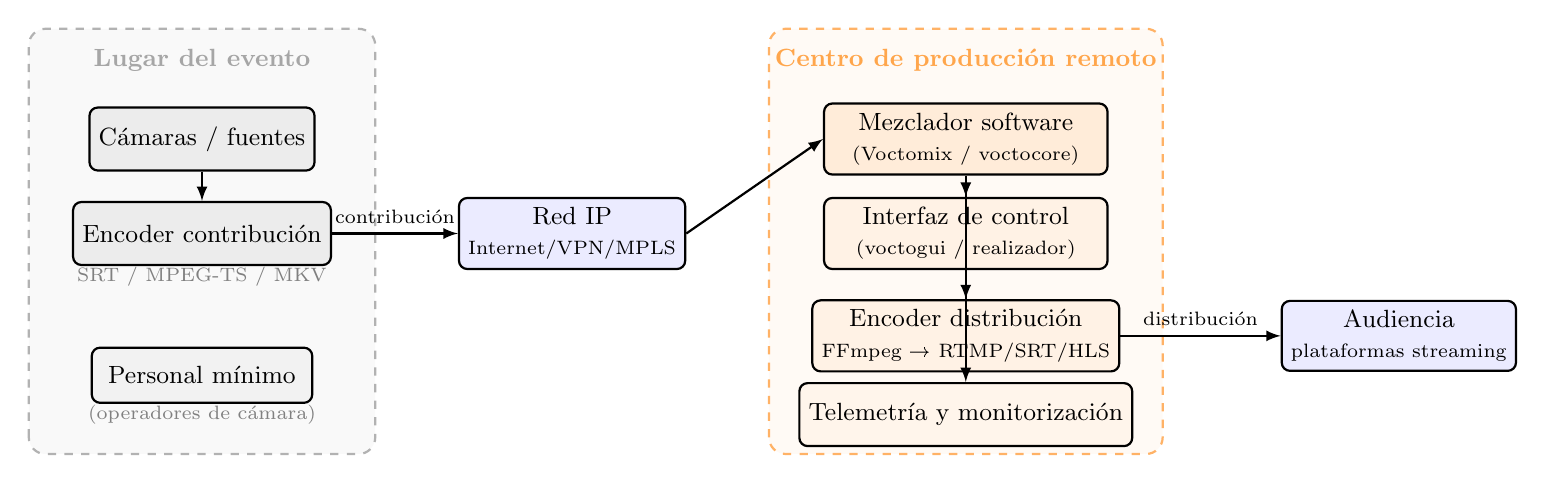
\begin{tikzpicture}[>=latex, thick, font=\small]
    % ── Lugar del evento (izquierda) ─────────────────────────────────
    \draw[rounded corners=6pt, dashed, gray!60, fill=gray!5]
      (-0.4,-2.0) rectangle (4.0,3.4);
    \node[font=\small\bfseries, gray!70] at (1.8,3.0) {Lugar del evento};

    \node[draw, rounded corners=3pt, minimum width=2.8cm, minimum height=0.8cm,
          align=center, fill=gray!15] (cam1) at (1.8, 2.0) {Cámaras / fuentes};
    \node[draw, rounded corners=3pt, minimum width=2.8cm, minimum height=0.8cm,
          align=center, fill=gray!15] (enc)  at (1.8, 0.8) {Encoder contribución};
    \node[font=\scriptsize, text=gray] at (1.8, 0.25) {SRT / MPEG-TS / MKV};
    \node[draw, rounded corners=3pt, minimum width=2.8cm, minimum height=0.7cm,
          align=center, fill=gray!10] (crew) at (1.8,-1.0) {Personal mínimo};
    \node[font=\scriptsize, text=gray] at (1.8,-1.5) {(operadores de cámara)};

    \draw[->] (cam1.south) -- (enc.north);

    % ── Red IP (centro) ───────────────────────────────────────────────
    \node[draw, rounded corners=3pt, minimum width=1.8cm, minimum height=0.8cm,
          align=center, fill=blue!8] (net) at (6.5, 0.8) {Red IP\\{\scriptsize Internet/VPN/MPLS}};
    \draw[->] (enc.east) -- (net.west)
      node[midway, above, font=\scriptsize] {contribución};

    % ── Centro de producción (derecha) ───────────────────────────────
    \draw[rounded corners=6pt, dashed, orange!60, fill=orange!4]
      (9.0,-2.0) rectangle (14.0,3.4);
    \node[font=\small\bfseries, orange!70] at (11.5,3.0) {Centro de producción remoto};

    \node[draw, rounded corners=3pt, minimum width=3.6cm, minimum height=0.8cm,
          align=center, fill=orange!15] (mix) at (11.5, 2.0)
          {Mezclador software\\{\scriptsize (Voctomix / voctocore)}};
    \node[draw, rounded corners=3pt, minimum width=3.6cm, minimum height=0.8cm,
          align=center, fill=orange!10] (gui) at (11.5, 0.8)
          {Interfaz de control\\{\scriptsize (voctogui / realizador)}};
    \node[draw, rounded corners=3pt, minimum width=3.6cm, minimum height=0.8cm,
          align=center, fill=orange!10] (dist) at (11.5,-0.5)
          {Encoder distribución\\{\scriptsize FFmpeg → RTMP/SRT/HLS}};
    \node[draw, rounded corners=3pt, minimum width=3.6cm, minimum height=0.8cm,
          align=center, fill=orange!8] (tel) at (11.5,-1.5)
          {Telemetría y monitorización};

    \draw[->] (net.east) -- (mix.west);
    \draw[->] (mix.south) -- (gui.north);
    \draw[->] (mix.south) -- ++(0,-0.3) -| (dist.north);
    \draw[->] (gui.south)  -- ++(0,-0.15) -| (tel.north);

    % ── Audiencia (derecha del centro de producción) ─────────────────
    \node[draw, rounded corners=3pt, minimum width=2.2cm, minimum height=0.8cm,
          align=center, fill=blue!8] (aud) at (17.0, -0.5)
          {Audiencia\\{\scriptsize plataformas streaming}};
    \draw[->] (dist.east) -- (aud.west)
      node[midway, above, font=\scriptsize] {distribución};
  \end{tikzpicture}
  \caption{Arquitectura del modelo REMI.}
  \label{fig:remi_arquitectura}
\end{figure}